\begin{event}{Computational Mathematics with Jupyter}{ICMS-Jupyter}{ICMS, Edinburgh, Jan. 16 -- 20, 2017}{USTAN,UPSud,USFD,UOXF,SOUTHAMPTON,UWarwick,Logilab,Simula,UGent}{47}{20}{https://opendreamkit.org/meetings/2017-01-16-ICMS/}

\textbf{Main goals.} The focus of the workshop was on various components from the Jupyter's ecosystem 
and related projects such as, for example, Jupyter notebooks kernels for mathematical software systems,
and their applications in research, training and teaching.

\textbf{ODK implication.} The workshop has been organised by Alexander Konovalov and Markus
Pfeiffer (USTAN). OpenDreamKit speakers included Marijan Beg, Mike Croucher, Jeroen Demeyer,
Hans Fangohr, Vidar Fauske, Alexander Konovalov and Markus Pfeiffer. Many other ODK members
were attending and took part in various activities taking place during the workshop.
The full list of participants is available at
\url{https://opendreamkit.org/meetings/2017-01-16-ICMS/participants/}.
The costs primarily included catering during the workshop and travel expenses.
Some expenses were covered by our partner project CoDiMa which supports computational
discrete mathematics community in the UK.

\textbf{Event summary.}

The workshop combined presentations and tutorials (mainly during morning sessions)
with concurrent coding and documentation sprints, which were advertised to the participants
to sign up. At the end of each day we heard brief reports from group activities.
The programme of the workshop is available
at \url{https://opendreamkit.org/meetings/2017-01-16-ICMS/programme/}. A very detailed
summary of the even is given by Raniere Silva (Software Sustainability Institute) and
Hans Fangohr at \url{https://www.software.ac.uk/blog/2017-02-07-computational-mathematics-jupyter}.

\begin{figure}[ht]
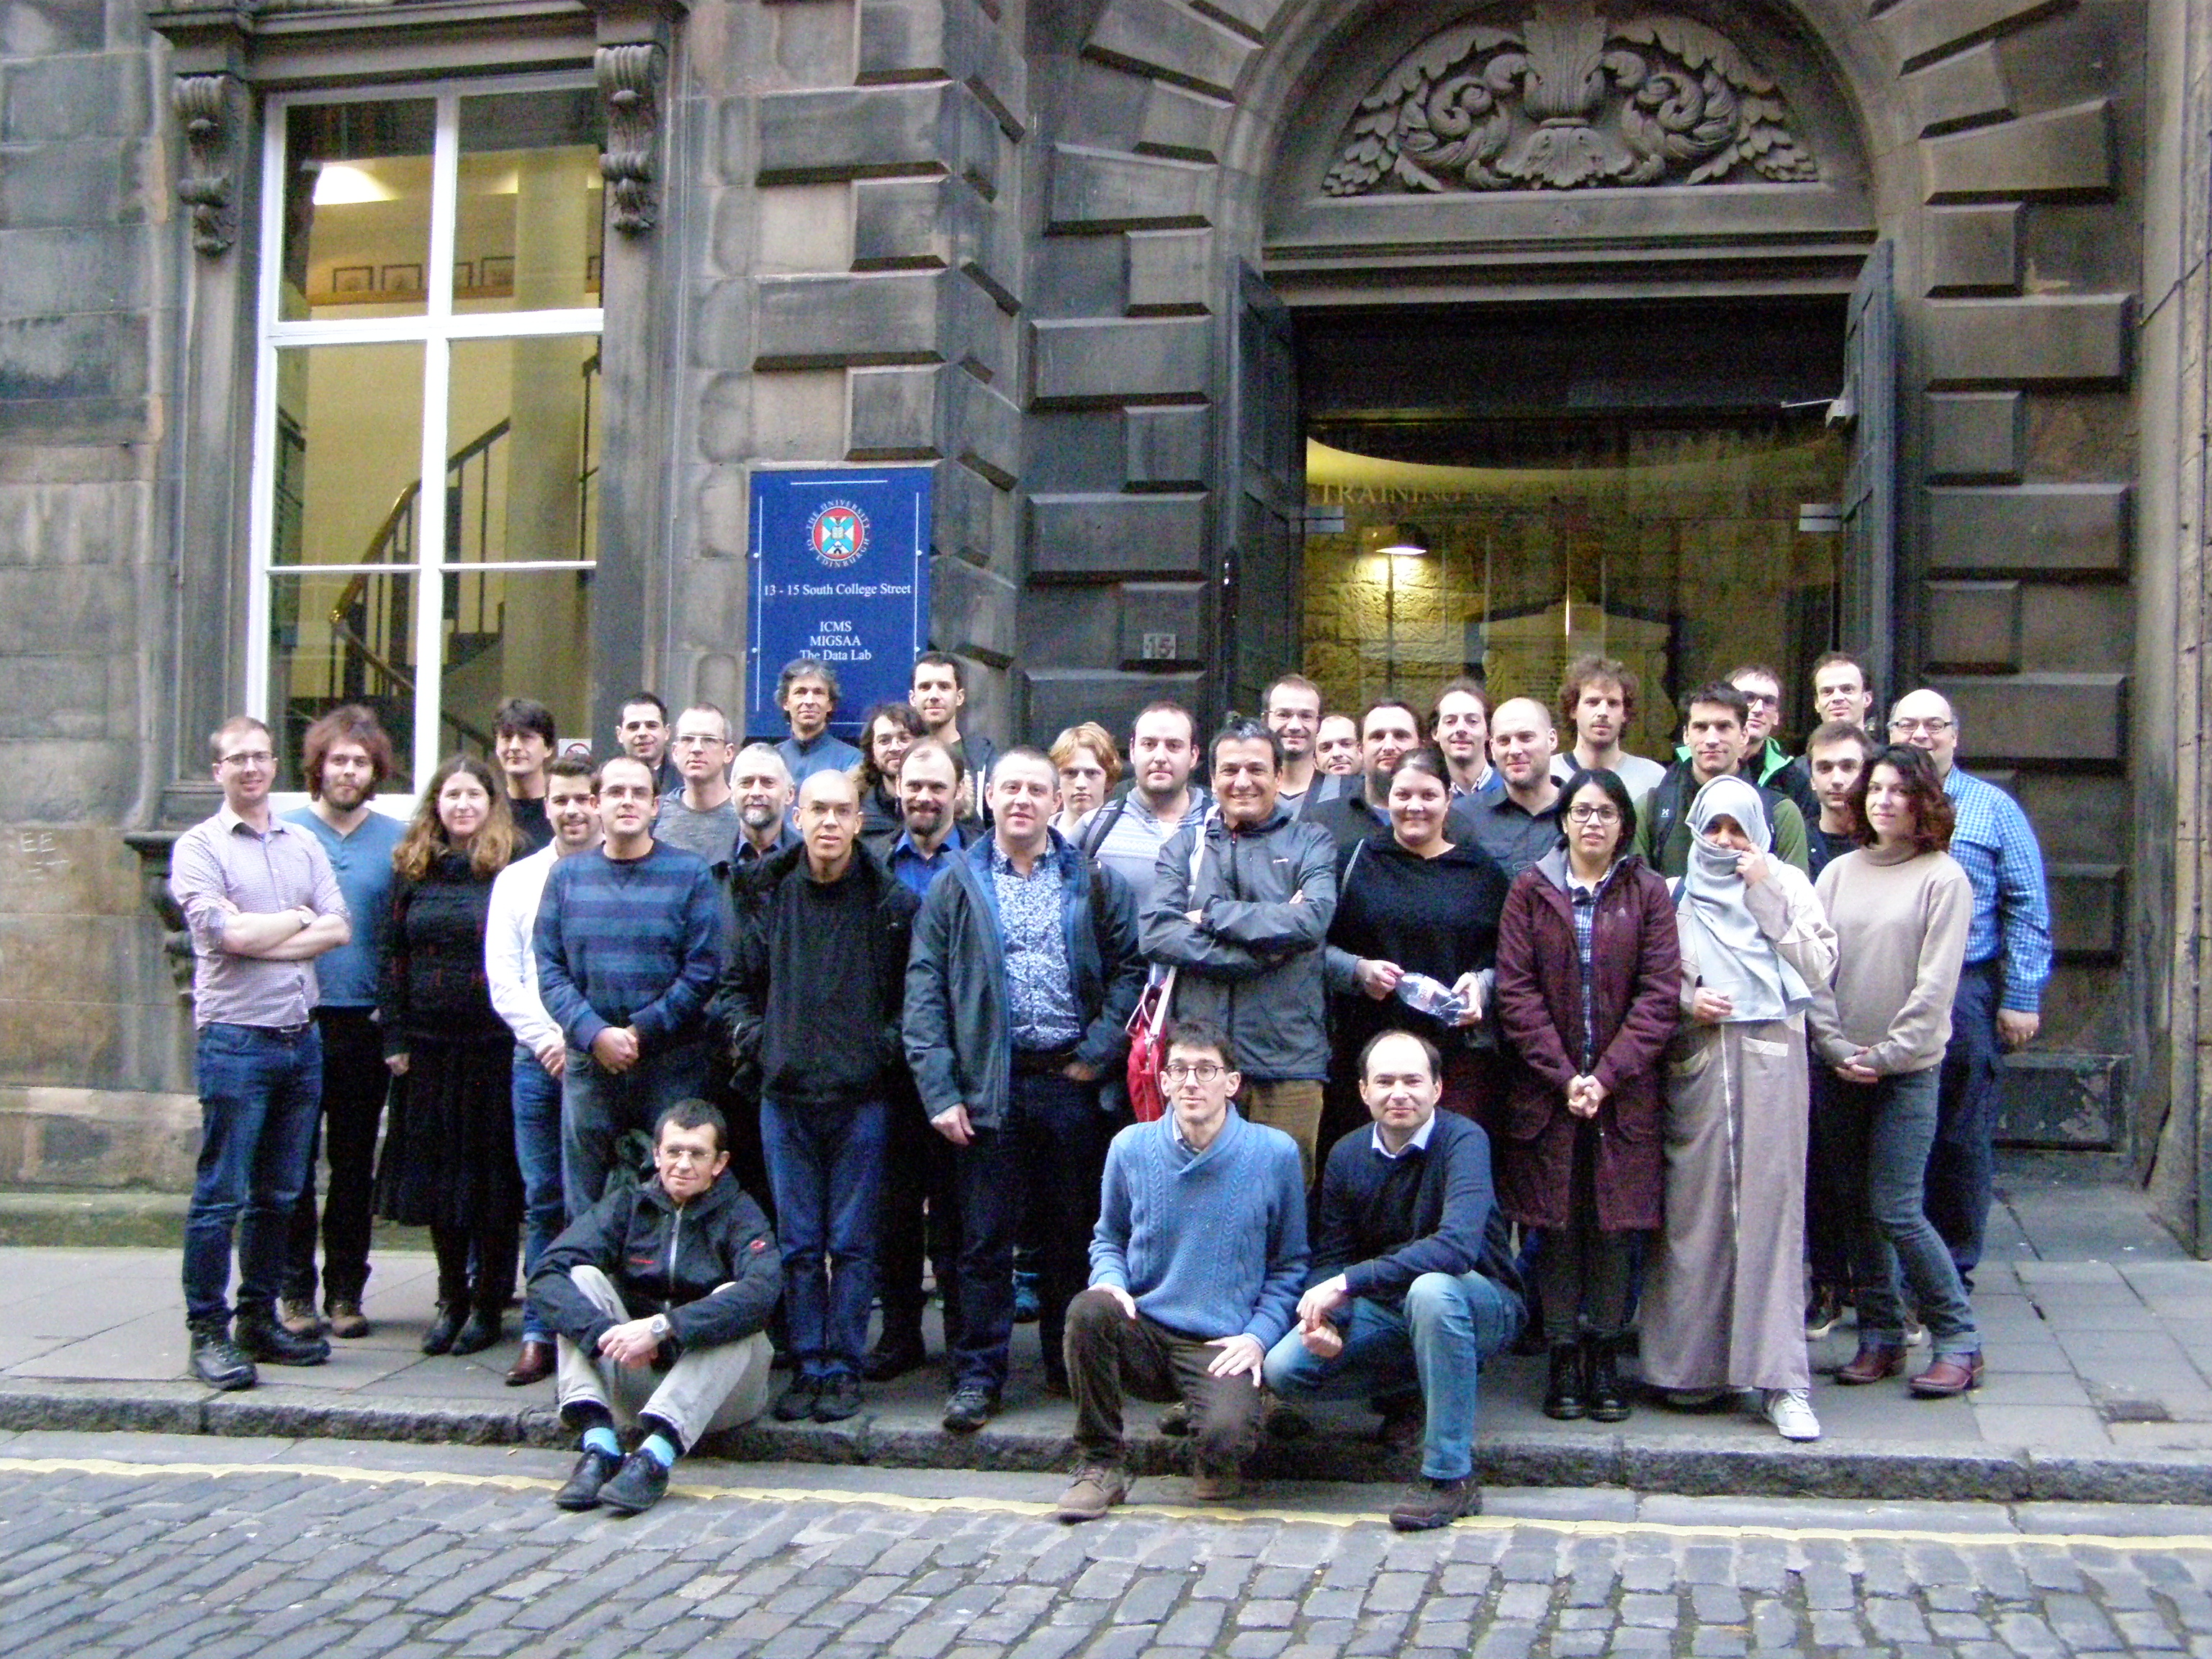
\includegraphics[scale=.14]{ICMS_Jan2017.jpg}
\caption*{Participants of the workshop ``Computational Mathematics with Jupyter''}
\end{figure}

\end{event}